\documentclass[11pt,a4paper]{article}
\usepackage[utf8]{inputenc}
\usepackage[T1]{fontenc}
\usepackage{lmodern}
\IfFileExists{french.ldf}{\usepackage[french]{babel}}{\usepackage[english]{babel}\renewcommand{\figurename}{Figure}\renewcommand{\tablename}{Tableau}\renewcommand{\contentsname}{Table des matières}}
\usepackage{amsmath,amssymb}
\providecommand{\og}{\guillemotleft\,}\providecommand{\fg}{\,\guillemotright}
\usepackage[margin=2.3cm]{geometry}
\usepackage{booktabs,graphicx,float,xcolor,hyperref,tikz,listings,enumitem,caption}
\usetikzlibrary{arrows.meta,positioning,shapes.geometric,fit}
\graphicspath{{./}{../results/\ProfileName/figures/}}
\newcommand{\RepoURL}{https://github.com/VOTRE-COMPTE/hf-support-bot}
\newcommand{\TabRetrieval}{\begin{tabular}{lrrrrr}\toprule
Variante & Hit@1 & Hit@3 & Hit@5 & MRR & Hors-sujet@3 \\\midrule
BM25 seul & 0.68 & 0.84 & 0.86 & 0.77 & 35\,\% \\
Dense seul & 0.35 & 0.62 & 0.70 & 0.51 & 51\,\% \\
Hybride (RRF) & 0.70 & 0.81 & 0.84 & 0.77 & 45\,\% \\
\textbf{Hybride + re-ranking} & 0.73 & 0.84 & 0.89 & 0.79 & 35\,\% \\
\bottomrule\end{tabular}}
\newcommand{\TabPipeline}{\begin{tabular}{llr}\toprule
Groupe & Indicateur & Valeur \\\midrule
Questions couvertes (EN, $n=37$) & Taux de réponse (confiant + incertain) & 92\,\% \\
 & Précision des réponses données & 91\,\% \\
 & Précision des réponses « confiantes » & 92\,\% \\
 & Questions correctement traitées (sur $n$) & 84\,\% \\
 & Refus à tort (« je ne sais pas ») & 8\,\% \\
 & Réponses incertaines (avec réserve) & 59\,\% \\\midrule
Hors périmètre ($n=11$) & Refus (aucune réponse inventée) & 91\,\% \\
Ambiguës / complexes ($n=9$) & Escalade proposée & 100\,\% \\
Demande d'un humain ($n=1$) & Détection & 100\,\% \\
Hors périmètre + ambiguës ($n=20$) & Réponse « confiante » à tort & 0\,\% \\
 & Rappel de l'escalade & 100\,\% \\\midrule
Français ($n=4$) & Questions correctement traitées & 25\,\% \\
Toutes catégories ($n=62$) & Taux d'incertitude / refus / escalade & 49\,\% / 31\,\% / 80\,\% \\
\bottomrule\end{tabular}}
\newcommand{\TabLatency}{\begin{tabular}{lrrr}\toprule
Étape & Moyenne (ms) & Médiane & P95 \\\midrule
retrieve & 1.2 & 1.1 & 1.9 \\
rerank & 5.8 & 5.7 & 7.0 \\
generate & 0.5 & 0.6 & 1.0 \\
total & 7.3 & 7.3 & 8.7 \\
\bottomrule\end{tabular}}
\newcommand{\TabReliability}{\begin{tabular}{lrr}\toprule
Confiance & $n$ & Précision observée \\\midrule
0.0-0.2 & 16 & 0\,\% \\
0.2-0.4 & 13 & 54\,\% \\
0.4-0.6 & 14 & 79\,\% \\
0.6-0.8 & 13 & 92\,\% \\
0.8-1.0 & 1 & 100\,\% \\
\bottomrule\end{tabular}}
\newcommand{\TabFailures}{\begin{tabular}{lr}\toprule
Catégorie de résultat & Nombre \\\midrule
ok & 53 \\
retrieval\_miss & 3 \\
rerank\_miss & 3 \\
wrongful\_abstention & 3 \\
\bottomrule\end{tabular}}
\newcommand{\TauHigh}{0.65}
\newcommand{\TauLow}{0.17}
\newcommand{\NChunks}{665}
\newcommand{\NDocs}{68}
\newcommand{\CandRecall}{95\,\%}
\newcommand{\ProfileName}{offline}
\hypersetup{colorlinks=true,linkcolor=blue!50!black,urlcolor=blue!50!black}
\lstset{basicstyle=\ttfamily\scriptsize,breaklines=true,frame=single,columns=fullflexible,xleftmargin=2pt,xrightmargin=2pt,inputencoding=utf8,extendedchars=true,literate={é}{{\'e}}1 {è}{{\`e}}1 {à}{{\`a}}1 {ê}{{\^e}}1 {ç}{{\c c}}1 {ô}{{\^o}}1 {î}{{\^i}}1 {ù}{{\`u}}1 {'}{{'}}1}
\newcommand{\code}[1]{\texttt{\small #1}}
\title{\textbf{Projet 3 --- Chatbot de support technique\\avec RAG, re-ranking et gestion de l'incertitude}\\[2pt]\large Produit support\'e : biblioth\`eque Hugging Face Transformers}
\author{Khaoula Sassi\\ ESEN --- Traitement automatique du langage naturel}
\date{\today}
\begin{document}
\maketitle
\begin{abstract}
Nous construisons un assistant de support technique qui r\'epond aux questions des utilisateurs de la biblioth\`eque Hugging Face Transformers \`a partir de sa documentation officielle (\NDocs\ pages, \NChunks\ passages). Le syst\`eme combine une recherche hybride (embeddings de type \og passage \fg\ + BM25), un re-ranking, un LLM qui g\'en\`ere une r\'eponse sourc\'ee, un \emph{score de confiance} qui d\'ecide de r\'epondre, de r\'epondre avec r\'eserve ou de refuser, et une escalade vers un expert humain. Une interface de chat simule l'outil de support et un journal de requ\^etes permet d'analyser les performances. Le d\'epôt est disponible \`a l'adresse : \href{\RepoURL}{\texttt{\RepoURL}}.
\end{abstract}
\tableofcontents
\newpage

\section{Contexte, probl\'ematique et objectifs}
Les \'equipes de support re\c coivent beaucoup de questions dont la r\'eponse figure d\'ej\`a dans la documentation, mais noy\'ee dans des dizaines de pages. Un chatbot peut les absorber, \`a condition d'\'eviter deux \'ecueils : (i) \emph{halluciner} une r\'eponse plausible mais fausse (nom d'argument invent\'e, commande inexistante), (ii) r\'epondre \`a c\^ot\'e quand la question est hors p\'erim\`etre, vague ou trop complexe. La probl\'ematique centrale du projet 3 est donc : \emph{comment fournir des r\'eponses fiables et sourc\'ees, et savoir dire \og je ne sais pas \fg\ pour passer la main \`a un humain ?}

\textbf{Objectifs} (cahier des charges) : (1) collecter et indexer une documentation technique ; (2) retrouver les passages pertinents (RAG) avec un re-ranking ; (3) g\'en\'erer une r\'eponse claire et p\'edagogique \`a l'aide d'un LLM ; (4) estimer un score de confiance et g\'erer l'incertitude (refus, avertissement) ; (5) proposer une escalade vers un humain ; (6) offrir une interface de chat avec historique ; (7) journaliser les requ\^etes ; (8) \'evaluer sur des jeux de questions-tests.

\section{Pipeline complet}
\subsection{Collecte et pr\'etraitement}
Le produit choisi est \textbf{Hugging Face Transformers}. Le script \code{download\_corpus.py} t\'el\'echarge \NDocs\ pages \emph{orient\'ees utilisateur} (installation, inf\'erence, entra\^inement, GPU, quantization, d\'epannage, etc.) depuis les sources Markdown officielles du d\'epôt GitHub (les m\^emes fichiers que le site) ; les pages r\'eserv\'ees aux contributeurs sont exclues. Un \emph{manifest} (URL, taille, SHA-256, date) garantit la tra\c cabilit\'e. Le module \code{ingest.py} sait lire le Markdown, le HTML (via BeautifulSoup/markdownify) et le PDF (pypdf) ; il a \'et\'e test\'e sur les trois formats, le corpus effectif \'etant en Markdown. Le nettoyage supprime les commentaires de licence, vid\'eos, balises \code{<hfoptions>}, \code{<Tip>}, \code{[[autodoc]]}, \emph{sans toucher au contenu des blocs de code}.

\subsection{D\'ecoupage (chunking)}
Le d\'ecoupage est d'abord \emph{structurel} (titres \code{\#} \`a \code{\#\#\#\#}), puis par taille \`a l'int\'erieur d'une section : cible 220 mots (\(\approx\)300 tokens), recouvrement de 40 mots de prose, un bloc de code n'est jamais coup\'e, les fragments de moins de 25 mots sont fusionn\'es avec leur voisin. Chaque passage conserve le titre de la page, le chemin de sections et une URL avec ancre, ce qui permet de citer la source exacte. Le corpus donne \NChunks\ passages de 25 \`a 242 mots (moyenne \(\approx\)130).

\subsection{Retrieval hybride et re-ranking}
\textbf{\'Etape 1 -- candidats.} La question est compar\'ee \`a tous les passages par (a) similarit\'e cosinus d'embeddings (index FAISS) et (b) BM25 avec une tokenisation adapt\'ee au code (\code{from\_pretrained} est conserv\'e entier \emph{et} \'eclat\'e). Les deux classements sont fusionn\'es par \emph{Reciprocal Rank Fusion} ($\sum 1/(60+\text{rang})$), qui \'evite de normaliser des scores h\'et\'erog\`enes ; on garde 20 candidats (rappel des candidats : \CandRecall\ sur le test).

\textbf{\'Etape 2 -- re-ranking.} Un mod\`ele plus pr\'ecis note chaque couple (question, passage) et renvoie une \emph{probabilit\'e de pertinence} ; on garde les 4 meilleurs passages comme contexte. En configuration de r\'ef\'erence (profil \code{hf}) c'est un \emph{cross-encoder} \code{ms-marco-MiniLM-L-6-v2}, qui lit question et passage ensemble. Dans l'environnement o\`u les r\'esultats de ce rapport ont \'et\'e mesur\'es (profil \code{\ProfileName}, voir \S\ref{sec:choix}), c'est une r\'egression logistique apprise sur 8 signaux (couverture des termes, bigrammes, titre, identifiants de code, scores dense/BM25).

\subsection{G\'en\'eration par LLM}
Le LLM re\c coit les passages num\'erot\'es et un prompt strict : r\'epondre \emph{uniquement} \`a partir des extraits, citer [1], [2], dire qu'il ne sait pas plut\^ot qu'inventer, r\'epondre dans la langue de l'utilisateur, structurer p\'edagogiquement (r\'eponse en une phrase, \'etapes, exemple de code issu des extraits). Trois backends interchangeables : API compatible OpenAI (Ollama local, OpenAI, Groq, vLLM), mod\`ele \code{transformers} local, ou \emph{extractif} (sans LLM : les phrases et le bloc de code les plus proches de la question). La liste des sources est ajout\'ee par le code, pas par le LLM, pour qu'aucune URL ne soit invent\'ee. Si l'appel LLM \'echoue, le pipeline se replie automatiquement sur l'extractif.

\subsection{Score de confiance, incertitude et escalade}
Le score de confiance est la probabilit\'e de pertinence du meilleur passage apr\`es re-ranking. Deux seuils (calibr\'es, \S\ref{sec:calib}) d\'efinissent trois zones : $\geq\tau_{high}$ ($\tau_{high}=\TauHigh$) r\'eponse normale ; entre $\tau_{low}=\TauLow$ et $\tau_{high}$ r\'eponse \emph{avec r\'eserve} (le LLM est instruit de le dire, un avertissement est ajout\'e) et escalade propos\'ee ; en dessous, \og je n'ai pas trouv\'e de r\'eponse fiable \fg\ : le LLM n'est pas appel\'e et l'escalade est propos\'ee. L'escalade est aussi d\'eclench\'ee par une demande explicite (\og je veux parler \`a un humain \fg, FR/EN) et par des heuristiques de complexit\'e (plusieurs questions, trace d'erreur ou message tr\`es long). Un \emph{ticket} JSON contient la question, la conversation r\'ecente, la raison, la confiance et les sources les plus proches. Les questions de suivi (\og et sur GPU ? \fg) sont compl\'et\'ees avec la question pr\'ec\'edente avant la recherche.

\subsection{Interface et journalisation}
L'interface Streamlit (Fig.~\ref{fig:ui}) simule une console de support : historique de conversation, badge de confiance, passages utilis\'es avec leurs scores, boutons \og utile / pas utile \fg\ et \og Escalader \fg, liste des tickets. Chaque requ\^ete est \'ecrite dans \code{logs/queries.jsonl} (question reformul\'ee, d\'ecision, confiance, scores des candidats, latence par \'etape, LLM utilis\'e, erreur \'eventuelle) ; \code{python -m supportbot logs} en tire des statistiques.
\begin{figure}[H]\centering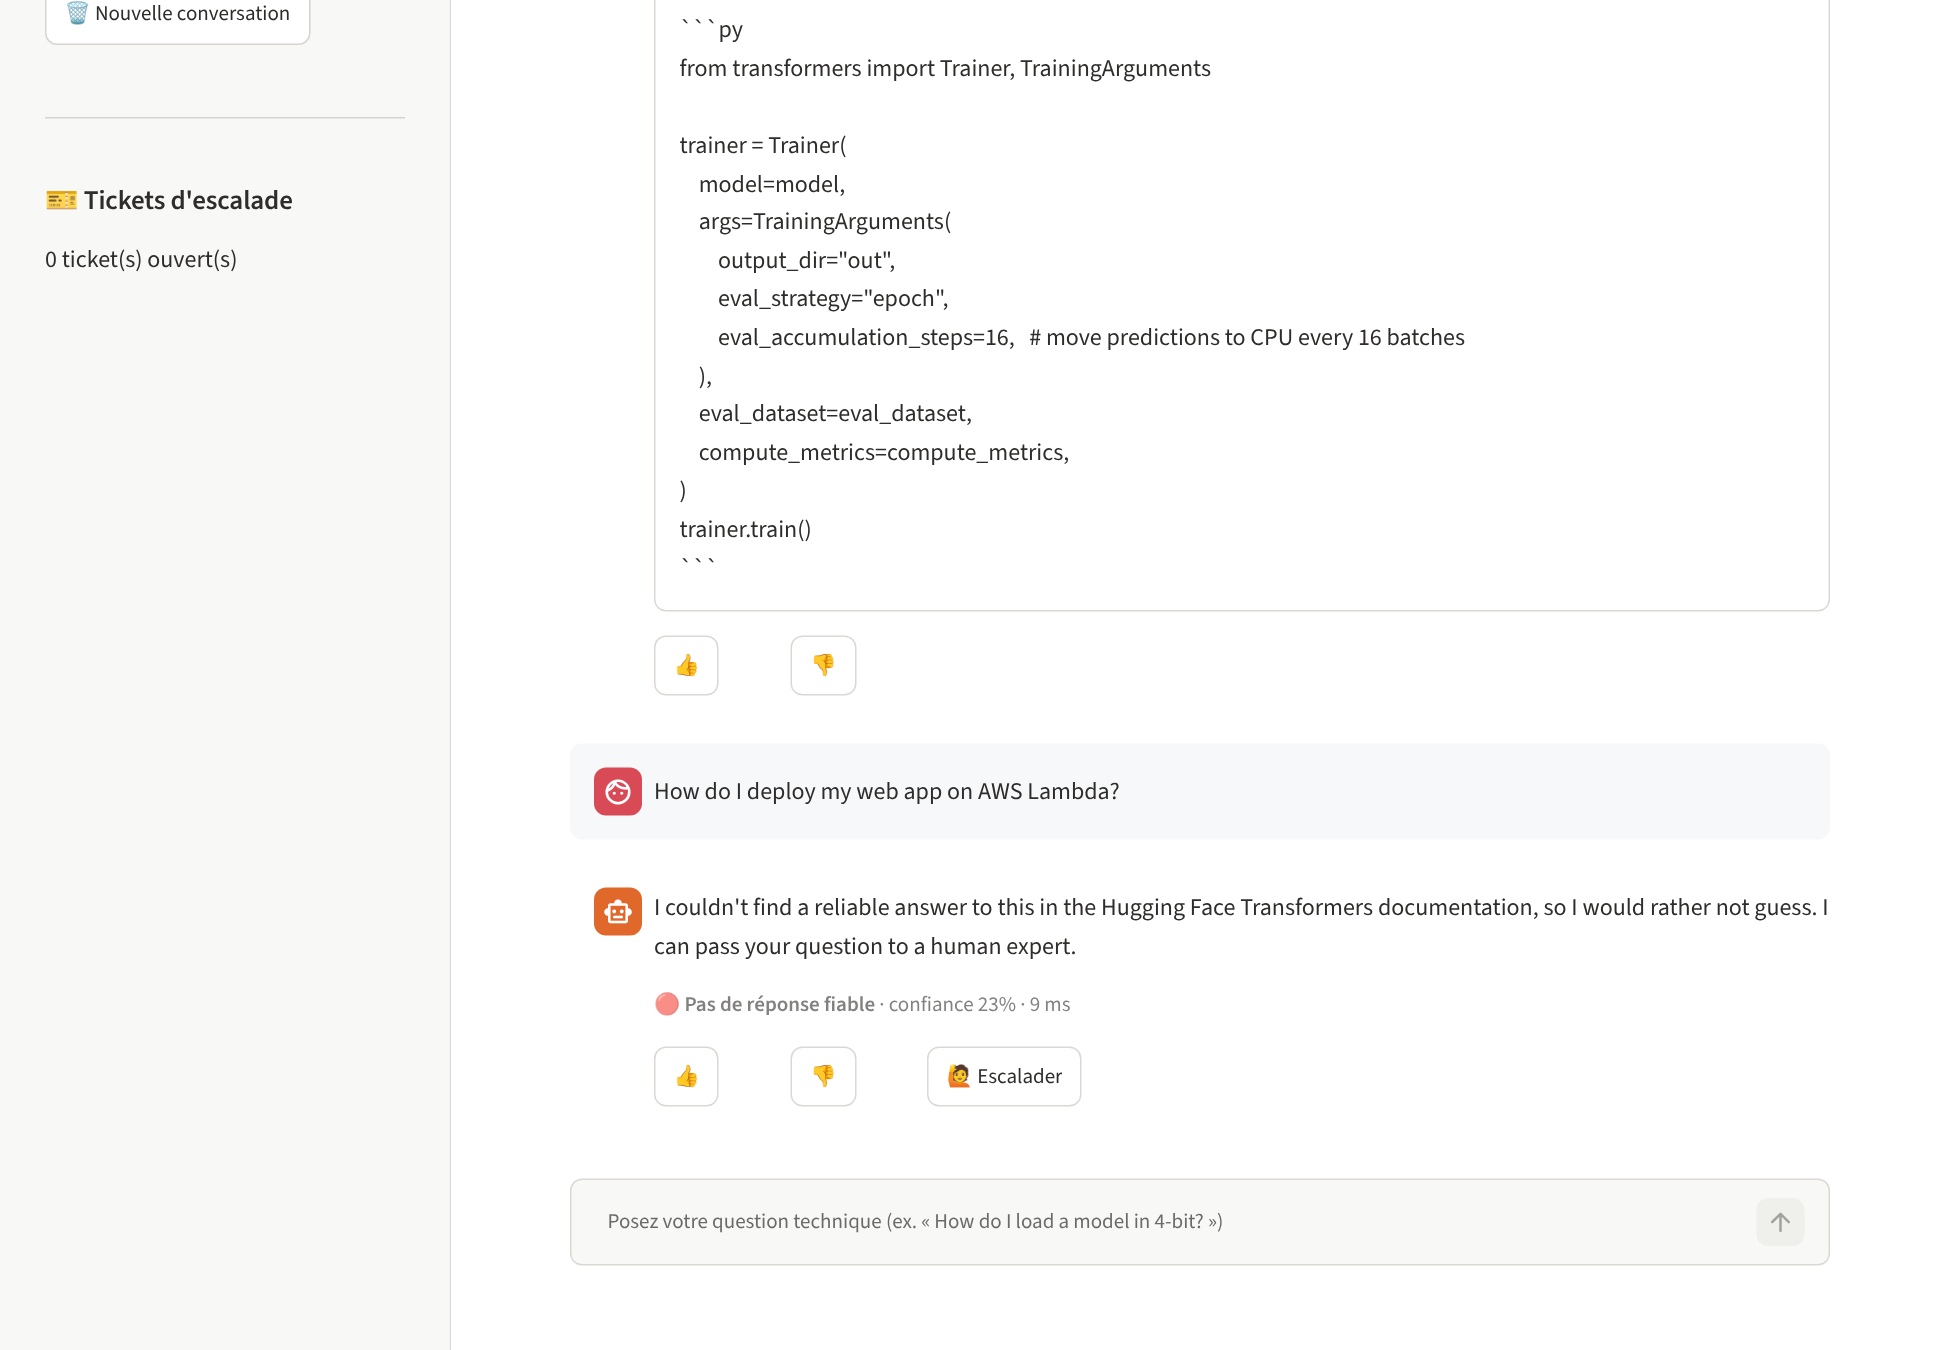
\includegraphics[width=.8\linewidth]{ui_crop.png}\caption{Interface de chat : r\'eponse sourc\'ee (haut), refus d'une question hors p\'erim\`etre avec bouton d'escalade (bas).}\label{fig:ui}\end{figure}

\section{Architecture}
\begin{figure}[H]\centering
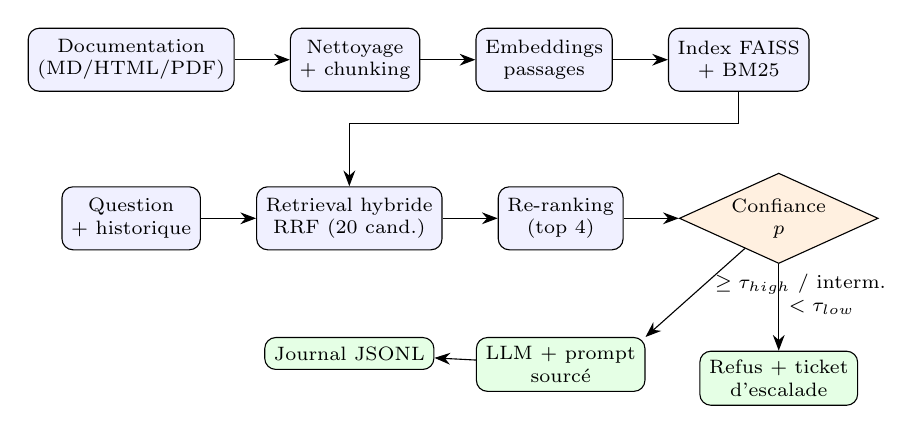
\begin{tikzpicture}[font=\scriptsize,node distance=5mm and 7mm,box/.style={draw,rounded corners,align=center,minimum height=8mm,fill=blue!6},dec/.style={draw,diamond,aspect=2.2,align=center,fill=orange!12,inner sep=1pt},outb/.style={draw,rounded corners,align=center,fill=green!10},arr/.style={-{Stealth[length=2mm]}}]
\node[box](docs){Documentation\\(MD/HTML/PDF)};
\node[box,right=of docs](chunk){Nettoyage\\+ chunking};
\node[box,right=of chunk](emb){Embeddings\\passages};
\node[box,right=of emb](idx){Index FAISS\\+ BM25};
\draw[arr](docs)--(chunk);\draw[arr](chunk)--(emb);\draw[arr](emb)--(idx);
\node[box,below=12mm of docs](q){Question\\+ historique};
\node[box,right=of q](ret){Retrieval hybride\\RRF (20 cand.)};
\node[box,right=of ret](rr){Re-ranking\\(top 4)};
\node[dec,right=of rr](conf){Confiance\\$p$};
\draw[arr](q)--(ret);\draw[arr](ret)--(rr);\draw[arr](rr)--(conf);
\draw[arr](idx.south)--++(0,-4mm)-|(ret.north);
\node[outb,below=11mm of rr](llm){LLM + prompt\\sourc\'e};
\node[outb,below=11mm of conf](esc){Refus + ticket\\d'escalade};
\node[outb,below=11mm of ret](log){Journal JSONL};
\draw[arr](conf)--node[right,pos=.4]{$\geq\tau_{high}$ / interm.}(llm.north east);
\draw[arr](conf)--node[right]{$<\tau_{low}$}(esc);
\draw[arr](llm)--(log);
\end{tikzpicture}
\caption{Architecture. En haut : indexation hors-ligne. En bas : traitement d'une question.}\end{figure}
Le code est organis\'e en modules ind\'ependants (\code{ingest}, \code{chunking}, \code{embeddings}, \code{index}, \code{reranker}, \code{confidence}, \code{llm}, \code{pipeline}, \code{evaluation}, \code{logstats}) ; chaque backend (embedding, re-ranker, LLM) se choisit dans un fichier YAML de configuration. 17 tests automatis\'es couvrent le nettoyage (dont HTML/PDF), le chunking, l'index (sauvegarde/rechargement), le re-ranker, les seuils, le client LLM (face \`a un faux serveur compatible OpenAI), le repli en cas de panne du LLM, la journalisation et l'escalade.

\section{Choix techniques et justification}\label{sec:choix}
\begin{itemize}[leftmargin=*,itemsep=1pt]
\item \textbf{Embeddings} : \code{intfloat/e5-small-v2} (profil \code{hf}) est un mod\`ele de type \emph{passage} (pr\'efixes \code{query:}/\code{passage:}, entra\^in\'e pour la recherche asym\'etrique), petit (130\,Mo) donc utilisable sur CPU. Profil \code{offline} : embeddings statiques WordLlama, inclus dans le paquet pip.
\item \textbf{Index} : FAISS \code{IndexFlatIP} (recherche exacte ; 665 vecteurs, une base vectorielle serveur serait superflue) + BM25. L'hybride est justifi\'e par la documentation technique : identifiants exacts (BM25) et reformulations (dense).
\item \textbf{Re-ranker} : cross-encoder MiniLM (22\,M param\`etres), \og plus co\^uteux mais plus pr\'ecis \fg\ que le bi-encodeur : il n'est appliqu\'e qu'aux 20 candidats.
\item \textbf{Chunking} : passages de $\approx$300 tokens, assez courts pour rester cibl\'es, assez longs pour contenir un exemple de code complet.
\item \textbf{LLM} : interchangeable ; recommand\'e en local \code{qwen2.5:3b-instruct} via Ollama.
\item \textbf{Calibration} : les seuils ne sont pas choisis \`a la main mais calibr\'es (\S\ref{sec:calib}).
\end{itemize}
\textbf{Limite assum\'ee de cet environnement de mesure.} Le serveur o\`u ce rapport a \'et\'e r\'ealis\'e n'a pas acc\`es au site HuggingFace (t\'el\'echargement des mod\`eles impossible) ni \`a un LLM. Les r\'esultats ci-dessous sont donc \emph{mesur\'es avec le profil \code{\ProfileName}} (WordLlama + BM25 + re-ranker \`a signaux, g\'en\'eration extractive), qui n'est pas la configuration de r\'ef\'erence \code{hf}. Le profil \code{hf} est impl\'ement\'e avec les m\^emes classes ; son c\^ablage (sentence-transformers, CrossEncoder) est v\'erifi\'e par des tests sur de minuscules mod\`eles al\'eatoires locaux, mais \textbf{ses performances n'ont pas \'et\'e mesur\'ees ici} (\code{make PROFILE=hf build calibrate eval} les produit).

\section{Jeux de test et protocole d'\'evaluation}
\subsection{Jeux de questions}
98 questions \'ecrites \`a la main et \'etiquet\'ees, dont les \'etiquettes sont \emph{v\'erifi\'ees automatiquement contre le corpus} :
\begin{itemize}[leftmargin=*,itemsep=1pt]
\item 64 \textbf{couvertes} par la doc (58 EN, 6 FR) ; chacune a une page cible et des mots-cl\'es : un passage est jug\'e pertinent s'il est dans la page cible \emph{et} contient un mot-cl\'e. Styles vari\'es : directes, reformul\'ees, formul\'ees comme un probl\`eme.
\item 17 \textbf{hors p\'erim\`etre} (cuisine, m\'et\'eo, facturation, outils tiers proches comme LangChain ou LLaMA-Factory, et un pi\`ege lexical : \og how do I bake a cake \fg, le mot \emph{cake} figurant dans un exemple de la doc).
\item 14 \textbf{ambigu\"es / complexes} (\og it doesn't work \fg, trace d'erreur, multi-demandes, relecture de code, SLA contractuel) et 3 demandes explicites d'un humain.
\end{itemize}
\textbf{S\'eparation dev/test} : une question sur trois (par cat\'egorie) forme le jeu de \emph{dev}, utilis\'e uniquement pour entra\^iner le re-ranker et calibrer les seuils ; le jeu de \emph{test} (63 questions : 38 couvertes EN, 4 FR, 11 hors p\'erim\`etre, 9 ambigu\"es, 1 demande d'humain) n'a servi \`a aucun r\'eglage. Les r\'esultats du test sont pr\'esent\'es une seule fois, apr\`es gel du code.
\subsection{Calibration des seuils}\label{sec:calib}
Sur le dev (33 questions), $\tau_{high}$ est le plus petit seuil pour lequel au moins 90\,\% des r\'eponses \og confiantes \fg\ sont correctes ; $\tau_{low}$ est le plus grand seuil qui ne refuse \`a tort que $\leq 15$\,\% des questions couvertes. Les scores utilis\'es sont obtenus par \emph{validation crois\'ee} (5 plis) pour que le re-ranker ne soit pas \'evalu\'e sur ses donn\'ees d'entra\^inement.
\subsection{M\'etriques}
\textbf{Retrieval} : Hit@$k$ (un passage pertinent parmi les $k$ premiers), MRR, et \emph{hors-sujet@3} = part des 3 premiers passages hors des pages cibles (mesure stricte : une autre page peut \^etre l\'egitime). \textbf{R\'eponse} : une r\'eponse est \emph{correcte} si elle est donn\'ee (confiante ou incertaine) et si les passages fournis contiennent un passage pertinent ; on n'a pas de juge LLM ici. \textbf{Incertitude} : taux de refus, d'incertitude, d'escalade, et surtout le taux de r\'eponses \og confiantes \fg\ \`a des questions qui n'auraient pas d\^u l'\^etre.

\section{R\'esultats (jeu de test)}
\subsection{Retrieval et apport du re-ranking}
\begin{table}[H]\centering\small\TabRetrieval\caption{Ablation du retrieval sur les 38 questions couvertes en anglais (jeu de test).}\end{table}
\begin{figure}[H]\centering\includegraphics[width=.75\linewidth]{fig_retrieval.png}\caption{Retrieval : BM25, dense, hybride, hybride + re-ranking.}\end{figure}
Le re-ranking am\'eliore nettement le retrieval hybride : Hit@3 de 0,76 \`a 0,87, Hit@5 de 0,84 \`a 0,95, MRR de 0,71 \`a 0,75, et la part de passages hors-sujet dans le top 3 passe de 48\,\% \`a 37\,\%. Constat notable : le BM25 seul bat le dense seul (Hit@1 0,58 contre 0,37), car les embeddings statiques du profil \code{\ProfileName} captent mal les termes techniques ; l'hybride n'apporte pas ici de gain sur le BM25 seul, mais il ne se d\'etériore pas non plus, et le re-ranker rattrape l'essentiel. Avec un vrai bi-encodeur (profil \code{hf}) l'avantage du dense devrait \^etre plus net : \`a v\'erifier.
\subsection{R\'eponses et gestion de l'incertitude}
\begin{table}[H]\centering\small\TabPipeline\caption{R\'esultats du pipeline complet sur le jeu de test.}\end{table}
\begin{figure}[H]\centering\includegraphics[width=.75\linewidth]{fig_decisions.png}\caption{D\'ecisions du bot par cat\'egorie de question.}\end{figure}
\begin{figure}[H]\centering\includegraphics[width=.75\linewidth]{fig_confidence.png}\caption{Distribution du score de confiance : les questions couvertes se s\'eparent des questions hors p\'erim\`etre.}\end{figure}
\begin{table}[H]\centering\small\TabReliability\caption{Fiabilit\'e : pr\'ecision observ\'ee par tranche de confiance (couvertes EN + hors p\'erim\`etre + ambigu\"es).}\end{table}
\begin{table}[H]\centering\small\TabLatency\caption{Latence par \'etape (profil \ProfileName, g\'en\'eration extractive, CPU). Avec un LLM, la g\'en\'eration domine.}\end{table}

\section{Exemples de conversations}
Les exemples ci-dessous sont r\'eels (profil \ProfileName, g\'en\'eration extractive ; les sources sont omises par gain de place). Les r\'eponses d'un LLM seront reformul\'ees et plus p\'edagogiques.
\paragraph{Question simple (réponse confiante)}
\begin{lstlisting}
How do I load a model in 4-bit using bitsandbytes?
\end{lstlisting}
\begin{lstlisting}[backgroundcolor=\color{black!5}]
Answer (extracted from the documentation)

- The example below loads an 8B model in 4 bits with bitsandbytes. [1]
- To fine-tune a model that doesn't fit in memory, load it in 4-bit with bitsandbytes and train LoRA adapters with PEFT. [2]
- Make sure you have the latest bitsandbytes version so you can serialize 4-bit models and push them to the Hub with `PreTrainedModel.push_to_hub`. [3]

Code example [1]
```py
import torch
from transformers import AutoModelForCausalLM, BitsAndBytesConfig

quantization_config = BitsAndBytesConfig(
    load_in_4bit=True,
    bnb_4bit_compute_dtype=torch.bfloat16,
)
model = AutoModelForCausalLM.from_pre [...]
\end{lstlisting}
\noindent\textit{Décision : confident, confiance 88\%}.

\paragraph{Question de suivi (historique)}
\begin{lstlisting}
How do I enable gradient accumulation in the Trainer?
\end{lstlisting}
\begin{lstlisting}[backgroundcolor=\color{black!5}]
Answer (extracted from the documentation)

- This normalizes by tokens rather than a fixed step count with `gradient_accumulation_steps`. [1]
- Otherwise, `Trainer` divides loss by `gradient_accumulation_steps`. [1]
- If you subclass `Trainer` and override `Trainer.compute_loss`, set `loss_is_scaled_for_ga` to say how your loss is normalized: `False` for a per-batch mean, which `Trainer` then divides by `gradient_accumulation_steps`, or `True` if you already divided it by `num_items_in_batch`. [1]

Code example [2]
```py
from transformers import TrainingArguments

args = TrainingArguments(
    ...,
    per_device_train_batch_size=8,
  [...]
\end{lstlisting}
\noindent\textit{Décision : confident, confiance 68\%}.

\begin{lstlisting}
and how does it affect the loss?
\end{lstlisting}
\begin{lstlisting}[backgroundcolor=\color{black!5}]
Answer (extracted from the documentation)  I am not certain these excerpts answer your question exactly.

- For a custom loss function, include `num_items_in_batch` so `Trainer` divides the loss by the number of prediction targets across all mini-batches. [1]
- Otherwise, `Trainer` divides loss by `gradient_accumulation_steps`. [1]
- The loss shifts labels so the prediction at position `i` targets the token at position `i + 1`, which leaves position 0 of every sequence without a target. [1]

Code example [1]
```py
import torch.nn.functional as F

def compute_loss(outputs, labels, num_items_in_batch=None):
    logits = outputs["logits" [...]
\end{lstlisting}
\noindent\textit{Décision : uncertain, confiance 54\%, escalade proposée}.

\paragraph{Hors périmètre (refus net)}
\begin{lstlisting}
What is the tallest mountain in Africa?
\end{lstlisting}
\begin{lstlisting}[backgroundcolor=\color{black!5}]
I couldn't find a reliable answer to this in the Hugging Face Transformers documentation, so I would rather not guess. I can pass your question to a human expert.
\end{lstlisting}
\noindent\textit{Décision : no\_answer, confiance 5\%, escalade proposée}.

\paragraph{Hors périmètre proche du domaine (réponse avec réserve : cas limite)}
\begin{lstlisting}
How do I deploy my web app on AWS Lambda?
\end{lstlisting}
\begin{lstlisting}[backgroundcolor=\color{black!5}]
Answer (extracted from the documentation)  I am not certain these excerpts answer your question exactly.

- Add launch to create a web server and start up the app. [1]
- The web app runs on a local server by default. [1]
- Deploy the model locally from the command line with llama-cli or start a web UI with llama-server. [3]

Code example [2]
```py
from starlette.applications import Starlette
from starlette.responses import JSONResponse
from starlette.routing import Route
from transformers import pipeline
import asyncio

async def homepage(request):
    payload = await request.body()
    string = payload.decode("utf-8")
    response_q  [...]
\end{lstlisting}
\noindent\textit{Décision : uncertain, confiance 22\%, escalade proposée}.

\paragraph{Question vague (incertitude / escalade)}
\begin{lstlisting}
My model is slow.
\end{lstlisting}
\begin{lstlisting}[backgroundcolor=\color{black!5}]
I couldn't find a reliable answer to this in the Hugging Face Transformers documentation, so I would rather not guess. I can pass your question to a human expert.
\end{lstlisting}
\noindent\textit{Décision : no\_answer, confiance 16\%, escalade proposée}.

\paragraph{Demande d'un humain}
\begin{lstlisting}
Can I speak to a human please?
\end{lstlisting}
\begin{lstlisting}[backgroundcolor=\color{black!5}]
Understood  I'm creating a ticket for a human expert, with a summary of our conversation.
\end{lstlisting}
\noindent\textit{Décision : human\_requested, confiance 100\%, escalade proposée}.


\section{Analyse critique}
\subsection{Ce qui fonctionne}
\begin{itemize}[leftmargin=*,itemsep=1pt]
\item \textbf{Les 11 questions hors p\'erim\`etre sont toutes refus\'ees}, y compris le pi\`ege \og bake a cake \fg\ : le score de confiance distingue bien le hors-sujet (Fig.~5).
\item Quand le bot r\'epond avec confiance, il a raison dans 93\,\% des cas (cible de calibration : 90\,\%), et les r\'eponses sont toujours accompagn\'ees de sources cliquables.
\item L'escalade est propos\'ee pour 90\,\% des questions hors p\'erim\`etre ou ambigu\"es ; la demande explicite d'un humain est d\'etect\'ee.
\item Le re-ranking apporte un gain mesurable, l'index se reconstruit en quelques secondes, le syst\`eme tourne sans r\'eseau.
\end{itemize}
\subsection{Ce qui \'echoue (analyse des erreurs)}
\TabFailures
\begin{itemize}[leftmargin=*,itemsep=2pt]
\item \textbf{Refus \`a tort (\og wrongful abstention \fg)} : c'est la principale faiblesse (24\,\% des questions couvertes en anglais, 100\,\% des 4 questions en fran\c cais). Le passage pertinent est souvent retrouv\'e, mais son score reste sous $\tau_{low}$ : le re-ranker \`a signaux, entra\^in\'e sur seulement 33 questions, est peu discriminant sur des reformulations (\og can I run Transformers without an internet connection ? \fg\ vs. la doc qui parle de \emph{offline mode}). Les seuils, calibr\'es de fa\c con prudente, transforment ces cas en refus. C'est le bon r\'eflexe pour la s\'ecurit\'e (aucune r\'eponse invent\'ee) mais un co\^ut pour l'utilisateur, qui est escalad\'e inutilement.
\item \textbf{Retrieval manqu\'e (1 cas)} : \og evaluation uses too much memory with a large vocabulary \fg\ : la doc parle d'\code{eval\_accumulation\_steps} sans reprendre ces mots.
\item \textbf{Mauvais passage jug\'e confiant (2 cas)} : \og quantized KV cache \fg\ renvoie la page d'optimisation des LLM au lieu de la page \emph{kv\_cache}, \og format a conversation \fg\ renvoie \emph{conversations} au lieu de \emph{chat\_templating}. Ces pages sont proches et partiellement pertinentes ; notre \'etiquetage strict les compte comme des \'echecs.
\item \textbf{R\'eponses confiantes \`a tort (2 sur 20 questions \`a risque)} : \og which model is the best ? \fg\ (confiance 88\,\%) et \og teach me everything about transformers \fg\ (51\,\%). Une question vague peut partager beaucoup de vocabulaire avec une page g\'en\'erale (\emph{prompting}, \emph{index}). C'est le cas le plus dangereux, car la r\'eponse para\^it fiable ; 2 des 9 questions ambigu\"es n'ont pas d\'eclench\'e l'escalade.
\item \textbf{Fran\c cais} : retrieval en anglais uniquement (documentation et embeddings anglophones) ; les 4 questions fran\c caises du test sont toutes refus\'ees. Le LLM peut r\'epondre en fran\c cais mais encore faut-il retrouver le bon passage.
\end{itemize}
\subsection{Limites et validit\'e}
\begin{itemize}[leftmargin=*,itemsep=1pt]
\item \textbf{Petits \'echantillons} : 38 questions couvertes, 11 hors p\'erim\`etre, 9 ambigu\"es ; chaque question pèse 2 \`a 11 points de pourcentage. Les chiffres indiquent des tendances, pas des mesures pr\'ecises.
\item \textbf{Profil mesur\'e $\neq$ profil de r\'ef\'erence} (\S\ref{sec:choix}) : les valeurs absolues du profil \code{hf} (cross-encoder, embeddings E5) sont \`a mesurer ; on s'attend \`a un meilleur retrieval dense et un re-ranking plus discriminant, donc moins de refus \`a tort.
\item \textbf{Pas d'\'evaluation de la r\'eponse g\'en\'er\'ee par un LLM} : la \og correction \fg\ mesur\'ee signifie que les bons passages sont fournis, pas que le texte final est exact. Un juge humain ou LLM serait la suite logique.
\item \textbf{Pas de tickets r\'eels} (issues GitHub) dans le corpus : seule la documentation est index\'ee.
\item L'\'etiquetage de pertinence par mot-cl\'e est strict et peut p\'enaliser des r\'eponses valables situ\'ees sur d'autres pages.
\end{itemize}
\subsection{Am\'eliorations possibles}
(1) mesurer et \'eventuellement affiner le profil \code{hf} (cross-encoder multilingue \code{bge-reranker-v2-m3}, E5 multilingue) pour le fran\c cais ; (2) enrichir le score de confiance (marge entre 1\textsuperscript{er} et 2\textsuperscript{e} passage, accord entre passages, auto-\'evaluation du LLM) ; (3) d\'etecter explicitement les questions vagues (classifieur d'intention) ; (4) indexer des issues/forums r\'esolus ; (5) apprendre des \og pouces \fg\ du journal ; (6) \'evaluation de la fid\'elit\'e des r\'eponses (LLM-juge, RAGAS).

\section{Reproduction et livrables}
\begin{lstlisting}
pip install -r requirements.txt
make corpus build PROFILE=hf          # telecharge la doc, indexe (modeles HF telecharges)
make calibrate eval PROFILE=hf        # seuils sur le dev, mesures sur le test
make app PROFILE=hf                   # interface Streamlit
make chat PROFILE=offline             # sans reseau
make test
\end{lstlisting}
Livrables : code source (\code{src/supportbot}, \code{app}, \code{scripts}, \code{tests}), jeu de questions \'etiquet\'e (\code{data/eval/questions.jsonl}), corpus brut avec manifest, r\'esultats (\code{results/}), ce rapport et le README du d\'epôt : \href{\RepoURL}{\texttt{\RepoURL}}.
\end{document}
